%!TEX root = origin_elements_lecture_notes.tex

\chapter{The Rapid Neutron Capture Process}

In 2020, 8.8\% of the total amount of energy produced in the United States originated from nuclear power plants.\footnote{\url{https://flowcharts.llnl.gov/commodities/energy}} These power plants use fissile uranium to heat water and create steam to run turbines in order to produce electricity. Uranium occurs naturally on Earth and can be mined. Its dominant isotope is \ex{238}U, which has a half-life of $4.468\times10^9$\,a and currently makes up most of the uranium on Earth, i.e., it has a relative abundance of 99.2742\%. The only other, naturally occurring uranium isotope is \ex{235}U with a relative abundance of 0.7204\%. Its half-life is $7.038\times10^8$\,a, which is long enough such that some of it is still alive after the 4.6\,Ga since the Solar System formation.

\section{Observations}\label{sec:r-process:observations}

The fact that the light turns on when we flip the switch shows that some process must exist that formed actinides prior to Solar System formation. 
\begin{figure}[tb]
    \centering
    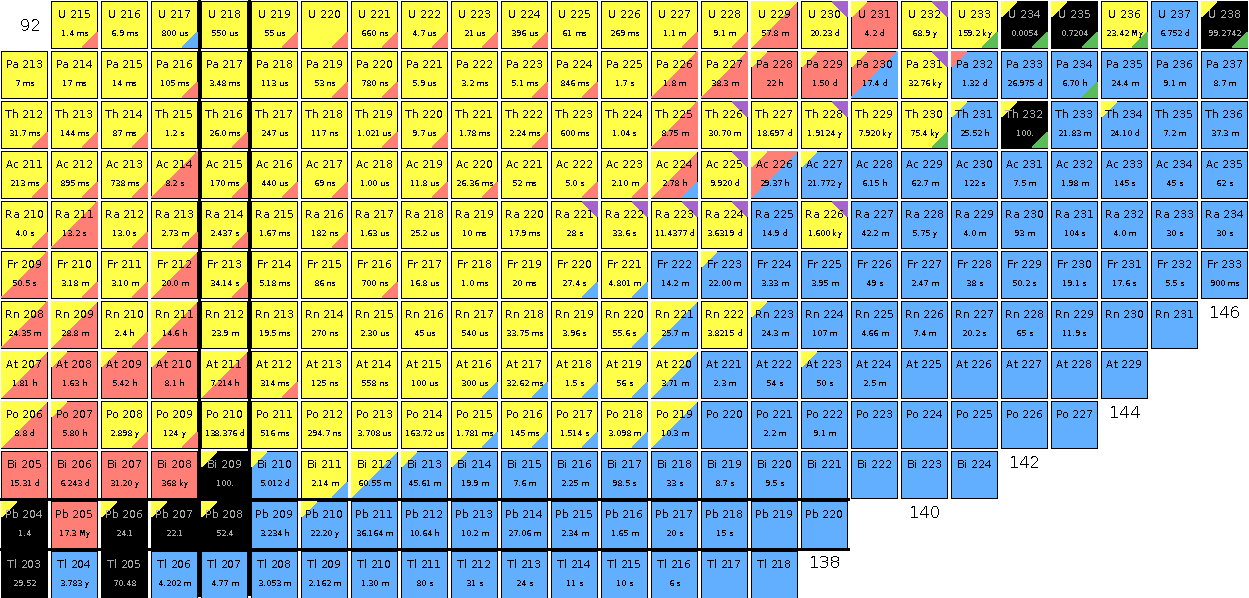
\includegraphics[width=\textwidth]{graphics/r-process/actinides_chartnuc}
    \caption{An excerpt of the chart of the nuclei, showing the lead and bismuth area which shows the end of the \ac{sproc}-path along with the actinides. Chart generated with a \href{https://github.com/kmiernik/Chart-of-nuclides-drawer}{python tool by Krzysztof Miernik}.}
    \label{fig:r-process:actinides_chart_nuclides}
\end{figure}
Figure~\ref{fig:r-process:actinides_chart_nuclides} shows an excerpt of the chart of the nuclides. On the left-hand side, the end of the \ac{sproc} can be seen at the stable lead and bismuth isotopes. The next, semi-stable isotopes that occurs naturally in the Solar System is \ex{232}Th with a half-life of $1.4\times10^{10}$\,a, which is about as long as the universe is old. To form \ex{232}Th by neutron capture, 23 neutrons would have to be captured on \ex{209}Bi without any decay in between. This is clearly not possible under \ac{sproc} conditions since the half lives of the unstable nuclei between \ex{209}Bi and \ex{232}Th are far to short. The actinides and other, neutron-rich nuclei therefore require another origin. 

\subsection{Solar System Abundances}

As for every process, the Solar System abundances (see Chapter~\ref{ch:solar_system_abundances}), are an important constraint in determining the relative proportions of the \ac{rproc}. Certain neutron-rich isotopes are completely shielded from being formed by the \ac{sproc}. For example, one such nucleus is \ex{130}Te. It is shielded from the \ac{sproc} path by the unstable \ex{129}Te (half-life 69.6\,min) and \ex{127}Te (half-life 9.35\,h). The latter nucleus in fact also effectively shields \ex{128}Te from the \ac{sproc}. Many more such nuclei can be found. 

\begin{figure}[tb]
    \centering
    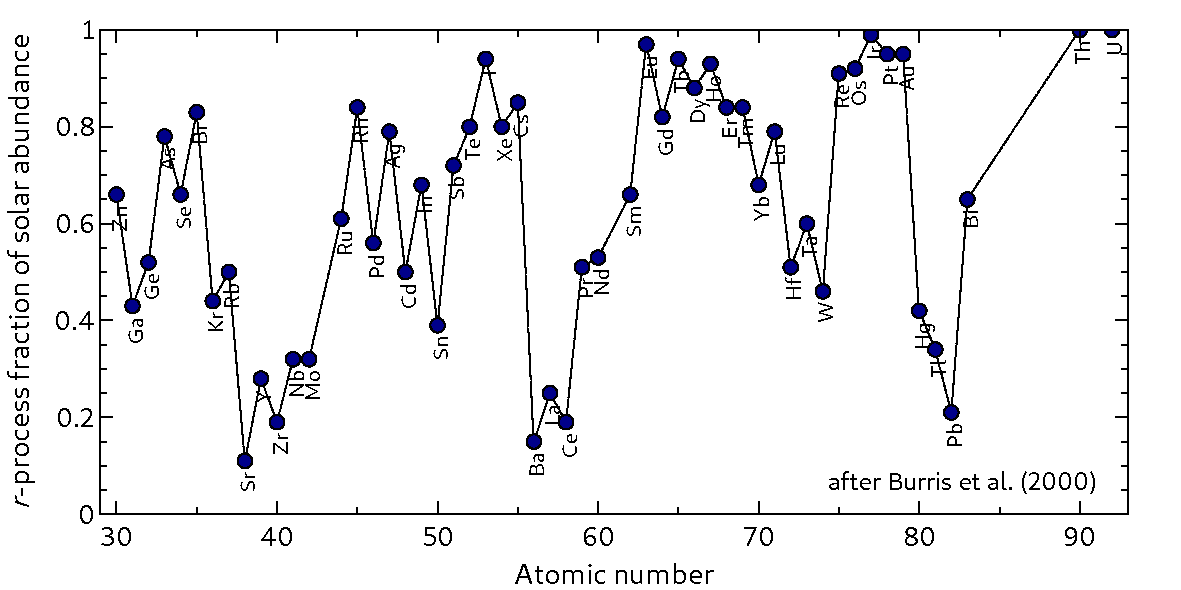
\includegraphics[width=0.85\textwidth]{graphics/r-process/rproc_abus}
    \caption{The \ac{rproc} fraction of the elements for elements heavier than strontium. Data from \citet{burris2000}.}
    \label{fig:r-process:r-process_fraction_solar_system_burris}
\end{figure}
Figure~\ref{fig:r-process:r-process_fraction_solar_system_burris} shows the \ac{rproc} fraction of the elements in the Solar System heavier than strontium. Here, the classical approach was taken in which the \ac{sproc} component was determined by fitting \ac{agb} star nucleosynthesis models to the measured solar abundances to explain the existence of \textit{s}-only nuclei. The \ac{rproc} abundance was then determined as the total solar abundance minus the \ac{sproc} contribution, i.e., as
\begin{equation}
    N_r(A,Z) = N_\odot(A,Z) - N_s(A,Z).
\end{equation}
Here, $N_r$, $N_s$ and $N_\odot$ are the respective abundances of an isotope with proton number $Z$ and mass $A$ for the \ac{rproc}, \ac{sproc}, and solar abundance, respectively. Half of the inventory of elements heavier than iron was made in the \ac{sproc}. Up to strontium, the weak \ac{sproc} mainly forms the elements, likely in massive stars, while the rest formed in the strong \ac{sproc} in \ac{agb} stars. Especially for the isotopes formed in the strong \ac{sproc}, the nucleosynthesis calculations are well constrained. 

The \ac{rproc} abundances show three distinct peaks. The first one is located around mass $A=82$, the second one around $A=130$, and the third \ac{rproc} peak around $A=195$. These peaks are direct consequences of the fact that the \ac{rproc} runs close to the neutron drip line.

\subsection{Ultra Metal-Poor Stars}

Figure~\ref{fig:r-process:r-process_fraction_solar_system_burris} shows that lanthanides are excellent \ac{rproc} proxies. For example, 97\% of the europium present in the Solar System is expected to have formed in the \ac{rproc}, making this element an excellent indicator for this process. In Chapter~\ref{sec:star_formation} we discussed the work of \citet{ji16}, who measured europium in Reticulum II. These measurements show that this ultrafaint dwarf was enriched by the \ac{rproc}, likely from only one single event. Otherwise, Reticulum II is rather metal poor, showing that the \ac{rproc} took place already early on in the galaxy. Thus, the astrophysical site must be able to come together within a short amount of time and the process can be expected to be of primary nature. Furthermore, the fact that Reticulum II has likely only been enriched by one single \ac{rproc} event sets a lower limit for the total amount of \textit{r}-nuclei ejected in it. These requirements put stringent constraints on potential astrophysical sites and on the \ac{gce} of \ac{rproc} elements. By observing the production timing and minimum mass of the ejected \textit{r}-nuclei, certain astrophysical sites such as regular \acp{sn} can be excluded from having enriched Reticulum II. In this specific case, \acp{sn} could account for the speed of the first \ac{rproc} enrichment, however, these events do not eject enough mass to account for the enrichment. 

As for most processes, we can assume that the \ac{rproc} likely takes place in more than one astrophysical location. Which astrophysical locations contribute and how much of the total amount of \textit{r}-nuclei they produce is recycled back into the galaxy is an active area of research. Only very limited direct observations that catch \ac{rproc} nucleosynthesis in the act exist. The most famous of these observations is linked to gravitational wave event GW170817, which was discovered by the \acf{ligo} on August 17, 2017. This gravitational wave event originated from two merging \acfp{ns}. Follow up spectroscopic observations showed the production of lanthanides, which are mainly produced in \ac{rproc} nucleosynthesis \citep{pian17}. These observations represent the first time that an actual \ac{rproc} event was observed in nature.


\section{Capturing Neutrons Rapidly}

We have seen in Chapter~\ref{ch:s-process} that the \ac{sproc} creates abundance peaks at neutron-magic numbers ($N=50, 82$, and 126). At these points, the neutron capture cross sections become small such that elements pile up and create abundance peaks in the \ac{sproc}. Similarly, the abundance peaks in the \ac{rproc} can be explained.

\subsection{Moving Towards and Along the Neutron Drip Line}

The \ac{rproc} is rapid since $\beta^{-}$ decays are always slower compared to capturing another neutron. Typical conditions, under which the \ac{rproc} can take place, are $T_9 \approx 1$ and a neutron density of $n_n \gtrsim 10^{20}\,\mathrm{cm}^{-3}$. Under these conditions, the relative abundance of an individual isotope $N(Z,A)$ can be determined by the equations for \acl{nse} as
\begin{equation}
    \frac{N(Z,A)}{N(Z,A+1)} = \frac{1}{n_n} \left(\frac{2\pi\mu kT}{h^2}\right) \frac{G_A G_n}{G_{A+1}} \exp\left(-\frac{Q_n}{kT}\right).
\end{equation}
Here, $\mu$ is the reduced mass of the neutron plus isotope ${^A}Z$, $k$ is Boltzmann's constant, $T$ is the temperature, and $h$ Planck's constant. The partition functions for nucleus ${^A}Z$ and the neutron are $G_A$ and $G_n$, respectively. Finally, $Q_n$ is the Q-value for a neutron capture on nucleus $^{A}Z$. The \ac{rproc} is a primary nucleosynthesis process, meaning that it can take place without the presence of any seeds.

\begin{figure}[tb]
    \centering
    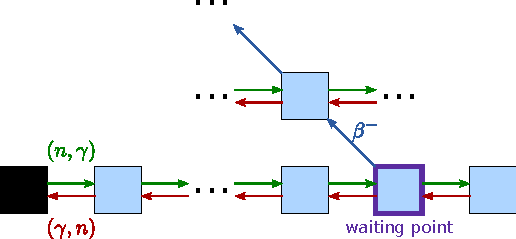
\includegraphics[width=0.75\textwidth]{graphics/r-process/rproc_schematic}
    \caption{Schematic of the \ac{rproc} capturing neutrons and halting at a waiting point.}
    \label{fig:r-process:schematic_waiting_point}
\end{figure}
Figure~\ref{fig:r-process:schematic_waiting_point} shows a schematic representation for rapid neutron capture from a stable nucleus (black). Blue nuclei are $\beta^{-}$ unstable, however, under \ac{rproc} conditions the possibility of capturing another neutron is higher than decaying along the isobar. At the temperatures at which the \ac{rproc} takes place, however, $(\gamma,n)$ processes can take place as well and destroy nuclei that formed by neutron captures. When the $(\gamma,n)$ and $(n,\gamma)$ reaction rates are equally likely, the \ac{rproc} reaches a so-called waiting point. At this point, the equilibrium
\begin{equation}
    (n, \gamma) \longleftrightarrow (\gamma, n)
\end{equation}
is maintained until the waiting point nucleus undergoes a $\beta^{-}$ decay along the isobar to the next element with $Z+1$ protons.

\begin{figure}[tb]
    \centering
    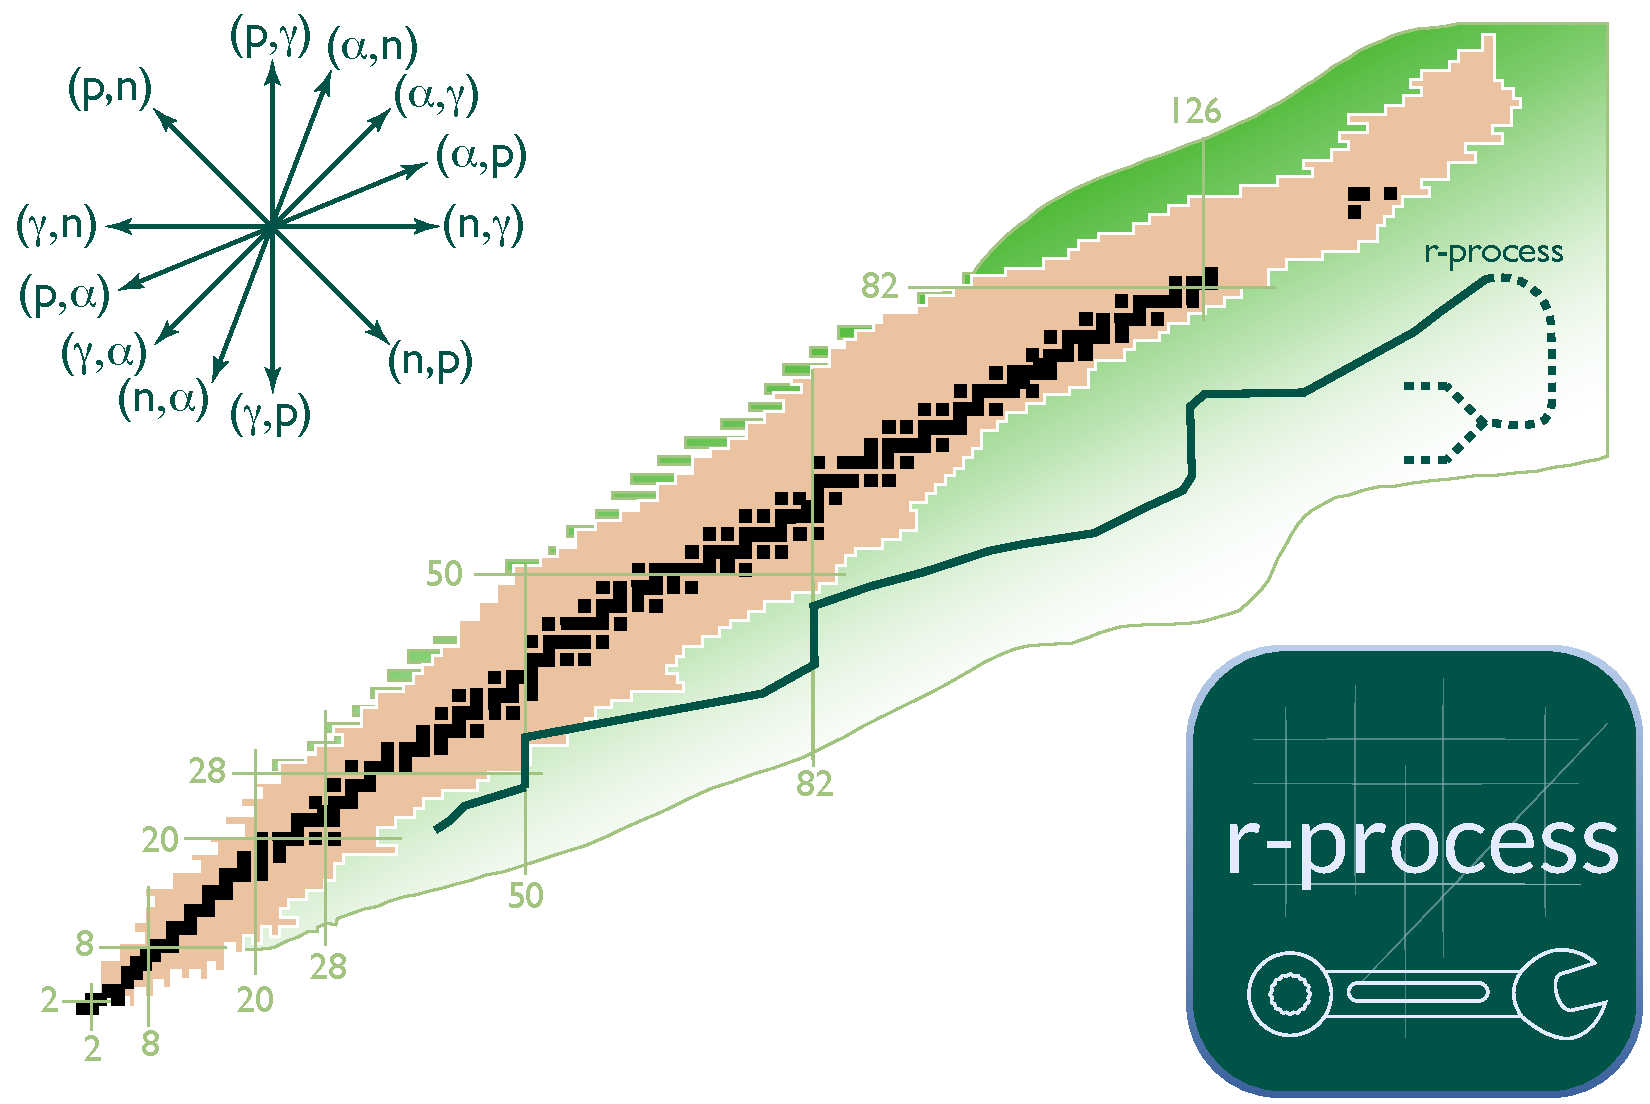
\includegraphics[width=\textwidth]{graphics/r-process/rproc_path}
    \caption{The path of the \ac{rproc}. Credit: Frank Timmes, Arizona State University, \url{http://cococubed.asu.edu/}.}
    \label{fig:r-process:rproc_path_timmes}
\end{figure}
The overall path of the \ac{rproc} is shown in Figure~\ref{fig:r-process:rproc_path_timmes}. At closed neutron shells, i.e., neutron-magic numbers, waiting points are reached and nuclei start piling up until $\beta^{-}$ decay can take place. This is shown by the horizontal path in the \ac{rproc} path in Figure~\ref{fig:r-process:rproc_path_timmes}. As discussed above, the \ac{sproc} also has a neutron capture bottleneck at neutron magic numbers which leads to abundance peaks at these masses. The same is the case for the \ac{rproc}, however, nuclei pile up far from the valley of stability in the neutron-rich region. Once the neutron source turns off, these isotopes decay back to the valley of stability. The discussed \ac{rproc} peaks, shown in Figure~\ref{fig:r-process:r-process_fraction_solar_system_burris} result from the decay of the isotopes that piled up at neutron magic numbers. Therefore, the \ac{rproc} peak abundances are shifted with respect to the \ac{sproc} ones.

\subsection{Fission Recycling}

Another important way of regulating the production of nuclei during the \ac{rproc} is fission recycling. Fission is a nuclear decay process in which an unstable nucleus breaks up into two or more lighter nuclei. While spontaneous fission takes place in nature, especially for very heavy isotopes, neutrons can also induce fission reactions. In fact, neutron-induced fission is used in nuclear power plants to generate heat. Here, \ex{235}U nuclei are irradiated with neutrons to induce fission, which breaks up the nuclei. These fission reactions are exothermic and release energy. The lighter nuclei that are formed include neutrons, which can then induce further fission reactions. In the extreme case scenario of a nuclear weapon, this can lead to a thermonuclear runaway. Nuclear power reactors contain neutron moderators that effectively suck up neutrons such that such chain reactions cannot take place.
\begin{figure}[tb]
    \centering
    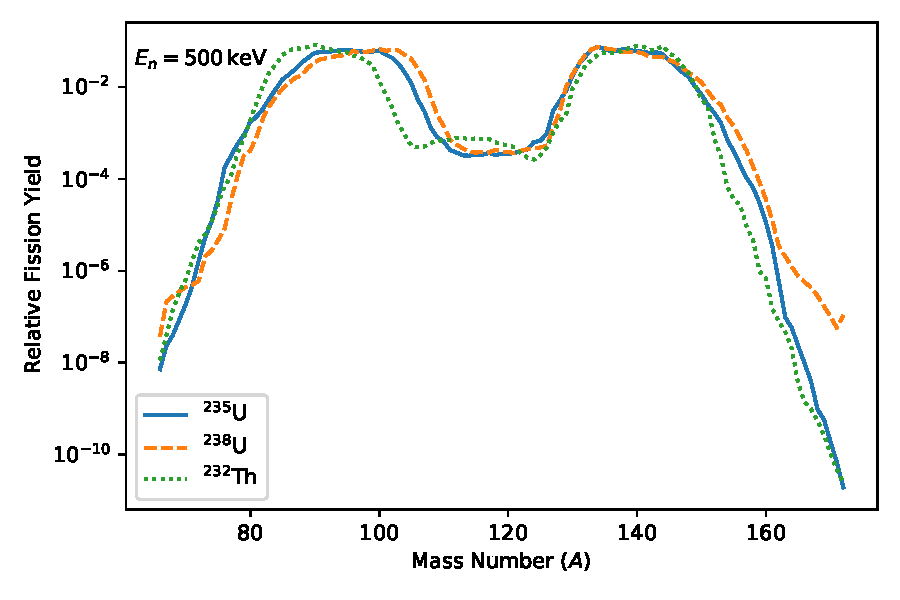
\includegraphics[width=0.75\textwidth]{graphics/r-process/fission_yield}
    \caption{The typical distribution of fission fragments from \ex{235}U, \ex{238}U, and \ex{232}Th, induced by $500\,keV$ neutrons.}
    \label{fig:r-process:fission_fragments}
\end{figure}
Figure~\ref{fig:r-process:fission_fragments} shows the fission fragments that are typically produced from uranium and plutonium. 

In the \ac{rproc}, very heavy elements such as actinides are formed by neutron capture. Since the \ac{rproc} necessarily takes place in a neutron-rich environment, fission reactions induced by neutron captures are expected. This effectively recycles part of the produced heavy nuclei back towards lower mass numbers, which is indicated by the dashed, green line at the end of the \ac{rproc} path in Figure~\ref{fig:r-process:rproc_path_timmes}.



\section{Astrophysical Sites}

While the underlying principals and conditions for the \ac{rproc} are well established, the astrophysical sites of the process2 are highly debated. Only one site has been observed so far that actively produced \textit{r}-nuclei, namely they \ac{ns}-\ac{ns} merger event GW170817\footnote{For details, see: \url{https://www.ligo.org/detections/GW170817.php}} first detected by \ac{ligo}. Other evidence for \ac{rproc} nucleosynthesis, see Section~\ref{sec:r-process:observations}, comes from observations of the results of \ac{rproc} nucleosynthesis in connection with \ac{gce} models. 

\subsection{Neutron Star Mergers}

Since the discovery of GW170817 and the follow-up observations that discovered the formation of \textit{r}-nuclei \citep{pian17}, \ac{ns} mergers have become one of the most favored astrophysical sites for explaining the \textit{r}-nuclei in the universe. While the observations clearly show that \ac{rproc} nucleosynthesis takes place in these events, it is still unclear if such mergers account for the whole inventory of \textit{r}-process nuclei in the universe.

\begin{figure}[tb]
    \centering
    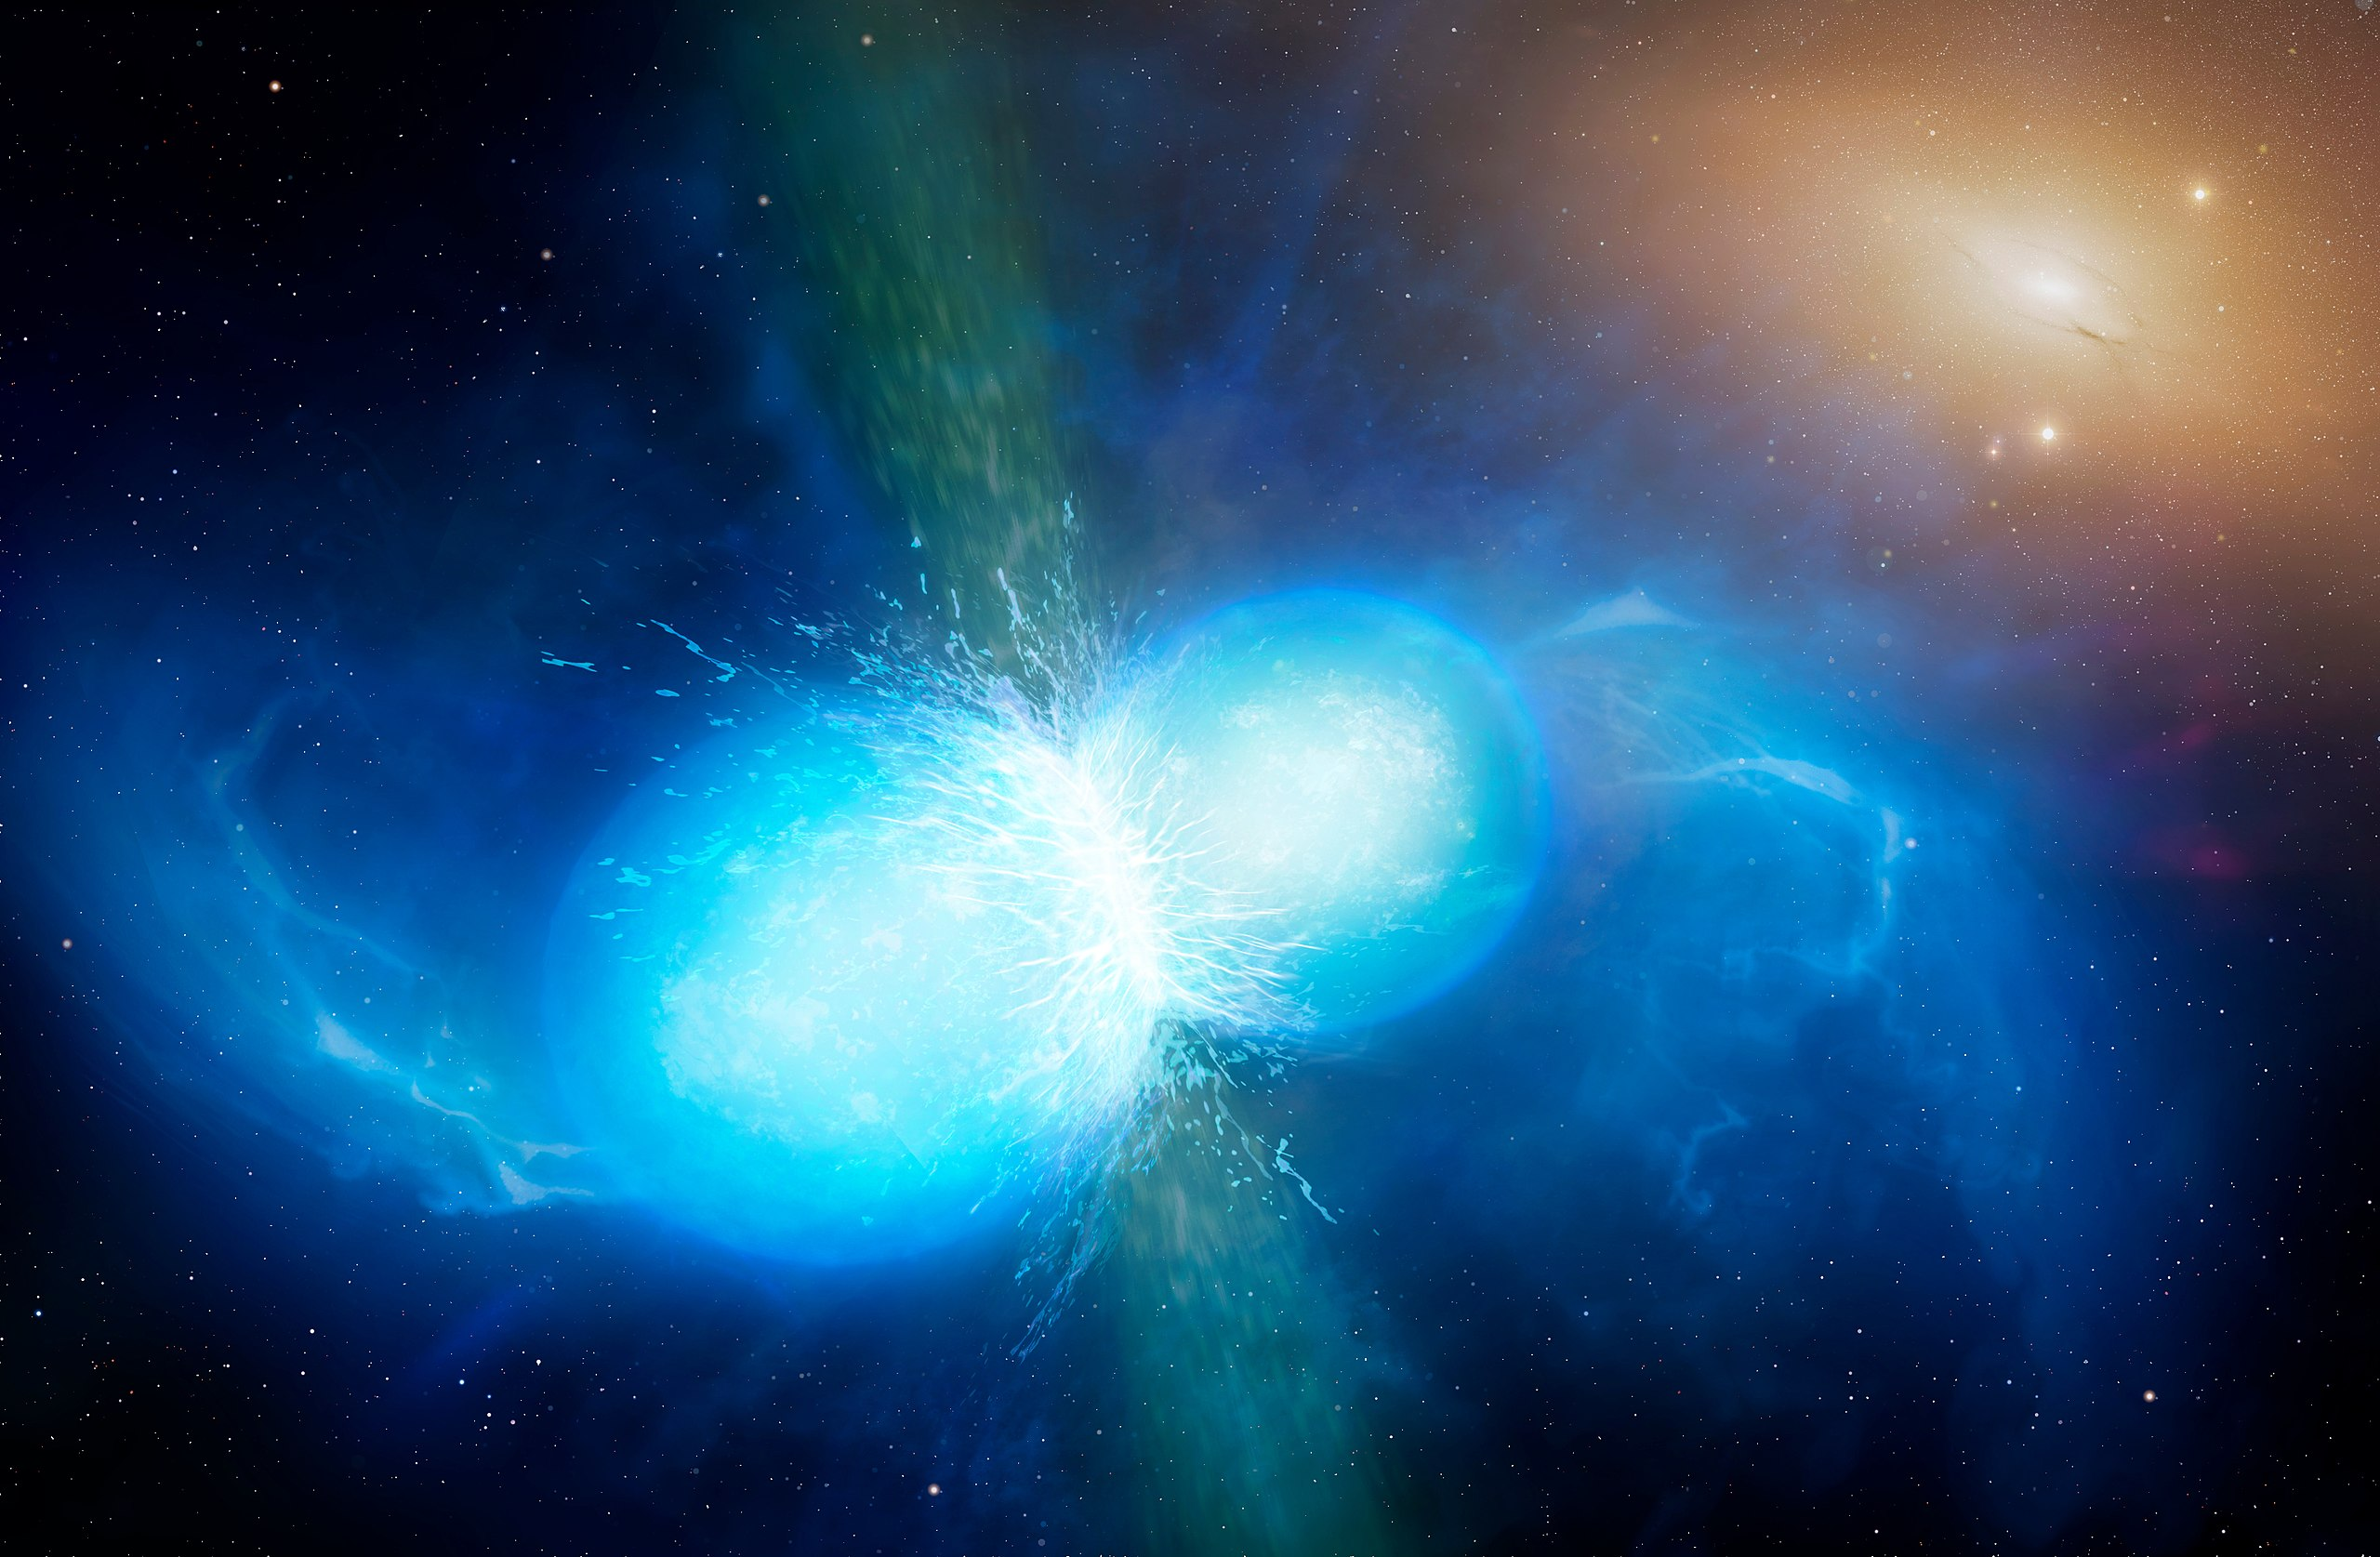
\includegraphics[width=0.75\textwidth]{graphics/r-process/ns-merger}
    \caption{Artist impression of \iac{ns}-\ac{ns} merger. Credit: \href{https://www.eso.org/public/images/eso1733s/}{University of Warwick/Mark Garlick}.}
    \label{fig:r-process:ns-merger}
\end{figure}
Figure~\ref{fig:r-process:ns-merger} shows an artist's impression of two merging neutron stars. Two orbiting neutron stars gradually loose energy by gravitational radiation. The gravitational waves that are finally released during the mergers were the ones that were detected by \ac{ligo} during GW170817. The energy release when merging also ejects a significant amount of matter, which can be very neutron rich. This allows the \ac{rproc} to take place during such events. Furthermore, it also recycles freshly nucleosynthesized \textit{r}-nuclei back into the Milky Way.

Current nucleosynthesis simulations of \ac{ns}-\ac{ns} mergers produce final abundances that are similar to the solar \ac{rproc} pattern, however, only for nuclei with masses $A>130$. The production of lighter nuclei is strongly influenced by nuclear fission and thus recycling of heavier elements. This recycling is highly dominated by uncertainties in the fission yields, thus making predictions of the \ac{rproc} patterns produced in such merger events uncertain.

In addition to \ac{ns}-\ac{ns} mergers, \ac{ns}-\ac{bh} mergers are also expected to produce \textit{r}-nuclei. Nucleosynthesis in these cases can take place in \ac{bh} accretion disks and subsequent \ac{rproc} nucleosynthesis products could be ejected by jets. Again, the exact pattern produced in these simulations highly depend on the model parameters.

\subsection{Supernovae}

Classical \acp{sn} have multiple times been proposed as the source of the \ac{rproc}, however, recent models seem to show that only light \textit{r}-nuclei might be produced in such events. The same reactions that contribute to the formation of the \textit{p}-nuclei can also create neutron-rich conditions, e.g., in neutrino-driven winds. Models show that the so-called weak \ac{rproc} can take place under these conditions which produces neutron-rich nuclei up to about $A\sim125$, see, e.g., \citet{shibagaki16}.

An additional possibility to form \textit{r}-nuclei in \acp{sn} is in neutron-rich material that is ejected into a jet. These magneto-hydrodynamic jet supernova models remain a viable astrophysical site for \ac{rproc} formation. Details on the models can, e.g., be found in \citet{winteler12}. Unfortunately, most of these jet simulations tend to under produce the nuclei just below and above the \ac{rproc} peaks.

\subsection{Collapsars}
Collapsars are failed \acp{sn} and represent a favored model for long-term \acp{grb} (see box below). In a collapsar event, a rapidly rotating, massive star collapses directly into a \ac{bh}. The angular momentum of the progenitor star leads to the formation of a heated accretion disk around the \ac{bh}. Jets allow the ejection of neutron-rich matter from the accretion disk along the polar axis. 

\begin{table}[bt]
\morebox{\Acl{grb}}{In the 1960s, the Vela series of military satellites were launched to check for compliance of the former Soviet Union with the 1963 nuclear test ban treaty. These satellites looked for $\gamma$-rays of terrestrial origin that would have originated from explosions of nuclear weapons. By 1967, military scientists had concluded that signals that were detected by these satellites did not come from the Earth below but rather the stellar events above. This information was not disclosed to the public until 1973. 

\acp{grb} happen around once per day in some random location in the sky. They last from around $10^{-2}$\,s up to $10^{3}$\,s and have very fast rise times of less than a tenth of a millisecond followed by an exponential decay of the signal. However, without knowing the distance to the origin of \acp{grb}, it was impossible to determine the processes that produced these events. The measured energy fluence for individual events ranges from $10^{-12}$\,J\,m$^{-2}$ up to $10^{-7}$\,J\,m$^{-2}$. In order to study \acp{grb}, the space shuttle Atlantis released on April 5, 1991, the \acf{cgro} in Earth's orbit. Several massive bursts were recorded by \acs{cgro}, among which was a \ac{grb} with a peak photon energy of 18\,GeV on December 15, 1994, which lasted for 90\,min. 

Ultimately, the successful combination of \ac{grb}-event detection in space with optical follow-up observations showed that \acp{grb} are of extragalactic origin. In fact, as for \acp{sn}, \acp{grb} are also dividable into two classes. Events that last longer than two seconds are referred to as long-soft \acp{grb} and are likely associated with \acp{sn}. Shorter events on the other hand are called short-hard \acp{grb} and seem to be associated with \ac{ns}-\ac{ns} or \ac{ns}-\ac{bh} mergers.}
\end{table}

Simulations of \ac{rproc} nucleosynthesis in collapsars showed that these events may supply up to 80\% of the of \textit{r}-nuclei in the universe \citep{siegel19}. In addition, collapsars form directly from one individual star and do not require two \acp{ns} or a \ac{ns} and a \ac{bh} to form first and then subsequently merge.

\subsection{Galactic Chemical Evolution}

Due to the lack of direct observations of \ac{rproc} nucleosynthesis sites, \ac{gce} models play a crucial role in understanding the formation of \textit{r}-nuclei in the universe. Several observations, such as Reticulum II, furthermore require \ac{rproc} nucleosynthesis to take place in the early universe. 

As for the \textit{p}-nuclei formation processes, no clear \textit{r}-only signature has been found in stardust grains. All stardust grains from \acp{sn} show a mix of various nucleosynthetic contributions, which is not surprising. After all, \acp{sn} are the host of the weak \ac{sproc} and might also be the sites for the $\gamma$- and the $\nu p$-process. To what matter the \ac{rproc} takes place in these objects is still a matter of debate. However, especially for the light \textit{r}-nuclei, the potential correlation of their origin with the \textit{p}-nuclei of the same element hints that \acp{sn} could in fact play an important role. A detailed discussion on this was already given in Section~\ref{sec:p-nuclei:observations}.

In addition to constraining the potential astrophysical site, \ac{gce} models can also constrain the frequency of the \ac{rproc}. This is especially important when comparing the initial Solar System abundances of \textit{r}-only nuclei such as thorium and uranium with the contemporary influx of these nuclei. As for recent contributions of \acp{sn} material to the Solar System (see Chapter~\ref{ch:massive_stars}), which can be seen in the terrestrial and lunar record by analyzing \acp{slr}, \textit{r}-only \acp{slr} can be used to determine the contemporary influx of, e.g., \ex{244}Pu. A recent study of deep-sea crust determined the current abundance of interstellar \ex{244}Pu on Earth \citep{wallner15}. This result showed a significantly lower abundance of contemporary \ex{244}Pu compared to the early Solar System. This indicates that \ac{rproc} nucleosynthesis takes place in rare events.

% FIXME This next section would benefit from a figure
As a rough estimate let us assume that the \ac{rproc} either takes place in \ac{ns} mergers or \acp{sn}. The latter are, according to observations, about 100 to 1000 times more frequent. Thus, the amount of \ac{rproc} nuclei ejected in \acp{sn} would be lower than the amount ejected by \ac{ns} mergers by about the same amount in order to account for the total \textit{r}-nuclei inventory of the Milky Way. Therefore, \acp{sn} would produce \textit{r}-nuclei constantly and the composition of \ac{rproc} \acp{slr} would reach a steady-state value in the galaxy. If \ac{ns} mergers on the other hand are the sole producers of \textit{r}-nuclei, the abundance of \acp{slr} in the galaxy produced in these events would be much more variable due to the low frequency of the events. The measurement of \citet{wallner15} has therefore been used in order to argue that \ac{rproc} nucleosynthesis of the actinides, i.e., the heavy \textit{r}-nuclei, takes place in rare events. Detailed \ac{gce} modeling on this has been performed by, e.g., \citet{bartos19}.


\section{Open Questions}

Many open questions remain with respect to \ac{rproc} nucleosynthesis, some of which have already been discussed. Two specific problems deserve special attention since solving these issues is crucial in furthering our understanding of this important nucleosynthesis process.


\subsection{The Europium Problem}

As already discussed, the ultrafaint dwarf galaxy Reticulum II shows stars with significant \ac{rproc} enrichments, even though these stars are old. The homogeneity of the signal furthermore indicates that only one single event contributed the \ac{rproc} nuclei in these galaxies, which excludes regular \acp{sn} as the producers of these nuclei since their ejected mass would not have provided enough \textit{r}-nuclei to explain this homogeneous signature. \citet{ji16} therefore concluded that another \ac{rproc} event must have contributed to Reticulum II. Europium, an \ac{rproc} element, has also been found to be present in ultra metal-poor halo stars. This means that \ac{rproc} nucleosynthesis must have taken place very early on in the history of the Milky Way in order to have contributed the products to these population II stars. However, evolving two massive stars into \acp{ns} and / or \acp{bh} and then merging them to produce \textit{r}-nuclei takes a significant amount of time. Single-star scenarios that can produce the \ac{rproc} would thus be preferable to solve this issue commonly referred to as the europium problem. Collapsars might therefore indeed play an important role in \ac{rproc} nucleosynthesis, however, without direct observations, these events remain mysterious.

\subsection{Terra Incognita}

The \ac{rproc} path takes place in very neutron-rich areas of the chart of the nuclides close to the neutron drip line. This poses significant challenges to nuclear physicists since reaction rate measurements for the involved isotopes are at the moment mostly impossible. The green-shaded area in Figure~\ref{fig:r-process:rproc_path_timmes} shows the so-called terra incognita. Here, nuclear experiments can currently not be performed since all the involved nuclei are too short-lived to be produced and studied in currently available laboratories. As Figure~\ref{fig:r-process:rproc_path_timmes} clearly shows, simulations of \ac{rproc} nucleosynthesis thus heavily rely on calculated nuclear masses and reaction rates. 

Currently under construction, the \acf{frib}\footnote{\url{https://frib.msu.edu/}} at Michigan State University in East Lansing, will allow researchers for the first time in the next years to access a large part of the terra incognita directly by experiments. These measurements will allow us to better determine the nuclear properties of isotopes involved \ac{rproc} nucleosynthesis and thus further our understanding of this elusive process.


\section{Reading}

For a detailed, recent review on \ac{rproc} nucleosynthesis, the reader is referred to \citet{kajino19}. This review article also discusses in detail the current situation around nuclear experiments and future opportunities with \ac{frib}.

The reading for this chapter focuses on the discovery of \ex{244}Pu in deep-sea sediments and crust material. Please read the article by \citet{wallner15}. This article discusses the measurement methods that led to the discovery of contemporary interstellar \ex{244}Pu in deep-sea crust. \citet{wallner15} also discuss the production scenarios and delivery of \ac{rproc} nuclei into the contemporary Solar System. The following bullet points might aid with the reading:
\begin{itemize}
    \item How does plutonium settle into the deep-sea sedmiments and into the ferromanganese crust? How fast do these individual depositions grow?
    \item What are the assumptions of \citet{wallner15} that go into modeling the incorportation of plutonium into the sea floor?
    \item What contamination do the measurements have to deal with and why?
    \item What are the assumptions that go into the models for \textit{r}-nuclei delivery into the contemporary Solar System?
    \item Are you convinced by the conclusions?
\end{itemize}